\documentclass[12pt,twoside,a4paper]{report}

\usepackage{amsfonts,amssymb,amsmath,epsfig}
\usepackage[portuguese,brazil]{babel}    % dá suporte para os termos na língua portuguesa do Brasil
%\usepackage[latin1]{inputenc} % dá suporte para caracteres especiais como acentos e cedilha
%\usepackage{ucs}
\usepackage[utf8]{inputenc}
\usepackage[T1]{fontenc}      % Lê a codificação de fonte T1 (font encoding default é 0T1).
\usepackage{ae}               % Fonte "Almost European"
%% \usepackage[portuguese]{babel}
%% %\usepackage[brazil,english]{babel}
%% %\usepackage[english,brazil]{babel}
%% \usepackage[T1]{fontenc}
\usepackage{indentfirst}
\usepackage{graphicx}

% ,fleqn] - Alinha as equações a esquerda ao invés de centraliza-las
%\setlength{\mathindent}{1cm} % determina o espaçamento entre a margem
                              % esquerda e as equações
                              
\usepackage{fancyhdr}
\usepackage[T1]{fontenc}
\usepackage{ae}
\usepackage{color}
\usepackage[printonlyused]{acronym}
%\usepackage{float} %put images where they are declared
%\floatplacement{figure}{H}
\usepackage{amsmath}
\usepackage{amsfonts}
\usepackage{hyperref}
%---- Tamanho das Paginas ----

%\oddsidemargin  =   2 mm
%\evensidemargin = -12 mm
\oddsidemargin  =  1 mm  %-5
\evensidemargin =  1 mm %-5
\textwidth      = 170 mm %170
\textheight     = 215 mm %235
\topmargin      = 8 mm %-10
\topskip        =  10  mm %10
\headsep        =  6 mm %10
\footskip       =   0 mm

%---- Espaçamento entre as linhas ----

\newcommand{\blst}{1.5} %{1.15}
\renewcommand{\baselinestretch}{\blst}

%---- Formato das Paginas ----

\pagestyle{headings}
\raggedbottom                 %  impede o ajustamento vertical

%---- Especificacoes sobre figuras ----

\setcounter  {topnumber}      {2}
\setcounter  {bottomnumber}   {2}
\setcounter  {totalnumber}    {2}
\renewcommand{\topfraction}   {1}
\renewcommand{\bottomfraction}{1}
\renewcommand{\textfraction}  {0}

%---- Formatando os títulos ----

\usepackage[bf,rm,compact]{titlesec}
\font\bigrm = cmr10 at 40pt
\titleformat{\chapter}[display]
            {\normalfont\huge\sffamily}
%            {\thispagestyle{empty}\normalfont\huge\sffamily}
            {\rightline{\normalfont\bigrm{\thechapter}}}
            {-2cm}
            {\bfseries}
            [{\vspace{-5mm}\hrulefill\\[.8ex]}]
\titlespacing{\chapter}
            {0cm}{0.5cm}{1.5cm}

%---- Headers ----

\usepackage{fancyhdr}
\pagestyle{fancyplain}
\renewcommand{\chaptermark}[1]{\markboth{\thechapter.\ #1}{} }
\renewcommand{\sectionmark}[1]{\markright{\thesection\ #1}}
\lhead[\fancyplain{}{\bfseries\thepage}]
       {\fancyplain{}{\small\slshape\bfseries\leftmark}}
\rhead[\fancyplain{}{\small\slshape\bfseries\rightmark}]
       {\fancyplain{}{\bfseries\thepage}}
\cfoot[\fancyplain{\bfseries\thepage}{}]
       {\fancyplain{\bfseries\thepage}{}}
\renewcommand{\headrulewidth}{0.3pt}

%---- Especificacoes Numeração ----

\setcounter{secnumdepth}{1}   %  numera apenas ate as seções
\setcounter{tocdepth}{1}      %  inclui no índice somente as seções

%%\input{hifen.tex}



\begin{document}

%%%%%%%%%%%%%%%%%%%%%%%%%%%%%%%%%
\pagestyle{plain}
%\pagenumbering{arabic}
\pagenumbering{roman}
\thispagestyle{empty}
\begin{center}

{\Large \sc
Universidade Estadual de Campinas \\
Instituto de Física {\em Gleb Wataghin} \\
\vspace{0.5cm}
F 896 - Monografia}

\vspace{2cm}

{\huge Estudo sobre

\bigskip

números mágicos dos \textit{clusters} de prata}

\vspace{2.5cm}

\end{center}

\begin{center}

{\large Maria Helena Gonçalves} \\
E-mail: mariahelenags10@gmail.com

\vspace{2.7cm}

%\noindent {\Large{Orientador:} Prof. Dr. Pedro Orientador} \\


%\vspace{1cm}


%\begin{tabular}{l}
{Orientador: Prof. Dr. Varlei Rodrigues}\\
E-mail: varlei@ifi.unicamp.br \\
Departamento de Física Aplicada \\
Instituto de Física {\em Gleb Wataghin}\\
Universidade Estadual de Campinas
%\end{tabular}

\end{center}

\vspace{0.5cm}

\begin{center}

\noindent {\Large{Campinas-SP}} \\
\noindent {\Large{\today}} \\

\end{center}

\newpage

$ $

\newpage

\chapter*{Resumo}
\markboth{Resumo}{Resumo}
\addcontentsline{toc}{chapter}{Resumo}

Na primeira parte d

\newpage

$ $
\newpage

\chapter*{Abstract}
\markboth{Abstract}{Abstract}
\addcontentsline{toc}{chapter}{Abstract}

In the first part 

\newpage

$ $
%\newpage

\chapter*{Biografia do Autor}
\markboth{Biografia do Autor}{Biografia do Autor}
\addcontentsline{toc}{chapter}{Biografia do Autor}

Concluí a escola média em 2010. Durante quatro anos trabalhei como webmaster
na empresa XXX, onde .... Iniciei o curso de física em 2013. Em 2015 como
aluno de iniciação científica e orientação do prof. Pedro Orientador
iniciei o desenvolvimento do projeto ... No final deste curso pretendo
buscar uma colocação em uma instituição financeira a fim de realizar
simulações de interesse no mercado acionário.

\newpage

$ $

\newpage

\vspace*{15cm}

{\large \hfill Dedico este trabalho}

{\large \hfill a .....}

\newpage

$ $

\newpage

\chapter*{Agradecimentos}

A meu orientador pela compreensão e dedicação com que orientou meu 
trabalho.

A meus amigos .....

\newpage

$ $
\newpage

\pagestyle{fancyplain}

\tableofcontents
%%%%%%%%%%%%%%%%%%%%%%%%%%%%%%%%%

%%%%%%%%%%%%%TEXTO%%%%%%%%%%%%%%%

\chapter{Introdução}
\pagenumbering{arabic}

A partir do fim da década de 70, os estudos de estruturas nanométricas começaram a ganhar destaque por sua relevância para a área da biomedicina. Duas décadas depois, o interesse em nanossistemas também ganhou força na área da física e, desde de então, os estudos nessa área cresceu em ritmo acelerado. As nanoestruturas apresentam propriedades novas e interessantes, que as diferem enormemente dos sistemas macroscópicos, e com grande potencial tecnológico em áreas como: química \cite{catalise}, eletrônica \cite{semicondutores} e biomedicina \cite{antimicrobial_effects, drug_delivery}.


Neste contexto, os nanoagregados, ou \textit{clusters} atômicos, são um caso interessante, pois podem ser compostos de dois a vários milhares de átomos, podendo ser formados por um ou mais elementos, e encontram-se na fronteira entre entre a física atômica e a física da matéria condensada.
%os átomos e o \textit{bulk}\footnote{\textit{Entende-se como "bulk" um conjunto de partículas sólidas grande o suficiente para que a média estatística de suas propriedades seja independente do número de partículas\cite{bulk}}}.
Seu estudo possibilita uma melhor compreensão de como as propriedades macroscópicas surgem do comportamento quântico da matéria \cite{Heer,Brack}.

As propriedades físico-químicas dos \textit{clusters} podem variar de forma abrupta com seu tamanho, principalmente quando se trata de \textit{clusters} atômicos, cujo diâmetro vária de $1-3$nm. Esse fato implica que é possível controlar essas propriedades se seu processo de formação for precisamente controlado  \cite{energetic_thermodynamic}, o que fomenta ainda mais o potencial tecnológico a essas estruturas.


Assim, uma das vertentes dos estudos realizados pelo Grupo   de   Física   de   Nanossistemas   e Materiais  Nanoestruturados  (GFNMN)  do  Departamento de  Física  Aplicada  (DFA),  são nanopartículas metálicas produzidas por uma Fonte de \textit{Clusters} e Agregados (FoCA). Este instrumento produz nano-partículas por um método físico, com controle de seu tamanho e de sua dispersão, além da sua composição. A FoCA foi desenvolvida por Artur Domingues Tavares de Sá e Giulia Di Domenicantonio \cite{tese_artur}, ex-membros do grupo, para possibilitar o estudo mais aprofundado das nanoestruturas.

Para obter a análise de distribuição de tamanho dos \textit{clusters}, por meio da distribuição de massa dessas partículas, é utilizado a técnica de espectrometria de massa por tempo de voo, possibilitando assim um estudo sobre suas propriedades em função do tamanho das partículas, o que torna a utilização dessa máquina muito interessante para o grupo.

% Esse tipo de análise permite que seja estudado critérios fundamentais para as tendências estruturais e energéticas.

Em um artigo seminal publicado por Knight \textit{et. al.} \cite{electronic_Shell_sodium}, medidas da distribuição de massas de \textit{clusters} de sódio ($Na$), produzidos em fase gasosa, mostra picos bem definidos e visivelmente maiores que os demais, para \textit{clusters} com $2, 18, 20, 34, 40, 58,92 ...$ átomos. Esses picos dizem respeito à maior abundância e estabilidade dos \textit{clusters} atômicos desses tamanhos em relação aos demais. Apelidou-se esses \textit{clusters} de "\textit{clusters} com números
\textit{mágicos} de átomos". A esses padrões foram atribuídos os efeitos de preenchimento das camadas eletrônicas \cite{Brack}. O modelo quântico de Jellium \cite{jellium} obteve sucesso para explicar os números \textit{mágicos}. Mas também existem casos em que \textit{clusters} \textit{mágicos} também aparecem devido ao preenchimento de camadas geométricas ou poliédricas, deixando de ser uma propriedade eletrônica.


Os números mágicos não aparecem somente para o elemento sódio ($Na$), mas sim para uma série de elementos incluindo os metais de transição como \cite{magic_1B}  cobre ($Cu$), prata ($Ag$), ouro ($Au$), platina ($Pt$) dentre muitos outros.

Um dos objetivos desse trabalho é utilizar a Fonte de \textit{Clusters} e Agregados e a técnica de espectrometria de massa por tempo de voo para estudar as tendências da abundância da formação dos \textit{clusters} de diversos tamanhos e tentar correlacionar com sua propriedades estruturais e energéticas. Pretende-se realizar experimentos com um metal de transição, no caso prata (\textit{Ag}), para verificar o aparecimento dos \textit{clusters} com números \textit{mágicos}. Além disso, os números mágicos também ocorrem no potencial de ionização dos agregados. Assim, pretendemos realizar experimentos com incidência de luz ultra violeta (UV), induzindo a sua ionização, e comparar os espectros de abundância obtidos com e sem o uso da luz UV. 

No capítulo 2 deste trabalho, serão  abordados os embasamentos teóricos sobre o aparecimento dos \textit{clusters} com números \textit{mágicos} sustentado pela literatura disponível. Subsequentemente, no capítulo 3 apresentaremos a máquina utilizada para a produção de \textit{clusters} e as modificações feitas na máquina para conseguir realizar os experimentos com luz UV. Discutiremos no capítulo seguinte as caracterizações
realizadas da prata e os resultados obtidos. Por fim realizaremos um
compêndio geral do trabalho apresentado, mostrando as principais conclusões. 



 
\chapter{Revisão Bibliográfica}
\label{revisao_bibliografica}

\section{Clusters}
\label{c2-clusters}

\textit{Clusters} são agregados de átomos ou moléculas, que variam desde dois à vários milhares de átomos e encontram-se na fronteira entre os átomos e o \textit{bulk}\footnote{\textit{Entende-se como "bulk" um conjunto de partículas sólidas grande o suficiente para que a média estatística de suas propriedades seja independente do número de partículas\cite{bulk}}}\cite{Heer,Brack}, por definição, eles se encontram em uma escala nanométrica ($ \leqslant 100$ nm).
No geral, os \textit{clusters} atômicos são classificados de acordo com seu tamanho: pequenos, médios ou grandes. Aglomerados classificados como pequenos, apresentam propriedades quânticas e possuem uma grande dependência com número de partículas que o compunha, essas propriedades não variam suavemente com seu tamanho, diferentemente dos \textit{clusters} médios e grandes. Normalmente os \textit{clusters} são ditos pequenos, quando contém mais do que algumas centenas ou quase mil partículas, os nano-agregados considerados grandes possuem muitas milhares de partículas e suas propriedades tendem a seguir as propriedades da matéria um \textit{bulk} \cite{livro_cluster}.


Deixando de lado os casos limites que geram ambiguidades, a diferença entre \textit{cluster} e moléculas encontra-se no fato que estas, no geral, possuem composições específicas e bem definidas e, na grande maioria dos casos, suas estruturas também são bem definidas, tendo  assim um número restrito de átomos; diferente de um \textit{cluster}, como exemplo podemos citar um \textit{cluster} de prata que pode conter de 2, 15, 100, ou qualquer outro número de átomos de prata respeitando os limites impostos para que este ainda seja um \textit{cluster}. Esses por sua vez também não possuem uma estrutura única, como podemos ver na Figura \ref{fig:estrutura_cluster_ag}, e para sua maioria, à medida que o número de partículas do \textit{cluster} aumenta, o número de estruturas estáveis disponíveis torna-se mais abundante. 

\begin{figure}
  \centering
  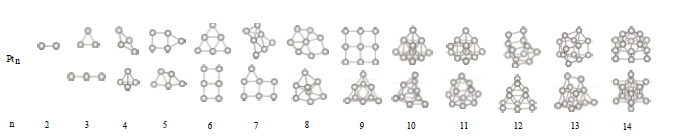
\includegraphics[width=1\textwidth]{images/clusters/estrutura_cluster_ag}
  \caption{ Exemplo de estruturas de \textit{clusters} de prata.\cite{dissertacao_anderson}  }
  \label{fig:estrutura_cluster_ag}
\end{figure}


O histórico de estudo da organização espacial dos arranjos atômicos frutificou em um Prêmio Nobel de Física em 1963. Metade do prêmio foi dado a Eugene Paul Wigner, por sua contribuição para a teoria do núcleo atômico e as partículas elementares,  e a outra metade foi partilhada por Maria Goeppert Mayer e J. Hans D. Jensen, pelas suas descobertas relativas à estrutura da casca nuclear. A análise das estruturas dos \textit{clusters} é fundamental para compreender suas propriedades e  dispor de seus potenciais tecnológicos, isso também torna-se muito importante para o domínio da estabilidade das nanopartículas. 


A análise da distribuição do tamanho dos \textit{clusters}, pode prover critérios fundamentais para o entendimento das tendências estruturais e energéticas e estruturais dos mesmos. Buscando entender melhor as transições das propriedades dos \textit{clusters}, segundo Bernd v. Issendorff (2009), podemos começar os estudos pensando em uma descrição simples, porém suficiente, do modo como se comportam os elétrons de um metal. Assumindo um sistema de elétrons livres, isto é, os elétrons da camada de valência se movem através de uma rede de metal infinita agindo como partículas livres. Assim, as funções de onda eletrônicas são apenas ondas planas tornando qualquer comprimento de onda possível.

Mudanças significativas ocorrem quando o metal possuí dimensões nanoscópicas ou são nanopartículas. Agora, as funções de onda formam ondas estacionárias entre as superfícies da partícula, o que é possível somente para certos comprimentos de onda. Uma consequência direta é a discretização da densidade eletrônica de estados: a banda de valência contínua se divide em um número infinito de estados. Este é o chamado efeito de tamanho quântico, que pode levar a mudanças significativas propriedades das partículas de metal. Pode-se esperar que tais efeitos possam ser mais claramente vistos para um metal que se aproxime do comportamento ideal dos elétrons livres \cite{capitulo_livro_shell}. A Figura \ref{fig:transicao_cluster_solido} mostra a mudança das propriedades de um material enquanto \textit{clusters} e enquanto sólido, ilustrando o que foi dito.

Uma das mudanças de propriedades interessantes é o surgimento de características semicondutoras em nanopartículas metálicas, que pode ser vista de Figura\ref{fig:carac_metal}. À medida que o número de átomos aumenta, também aumenta o número de níveis de energia disponíveis, até que a divisão entre níveis ocupados e desocupados se torna muito próxima e o \textit{cluster} começa a exibir comportamento metálico. Se aumentarmos um pouco o tamanho desta nanopartícula essas começaram a exibir comportamentos de pequenos pedaços do metal macroscópico. Abaixo desse tamanho crítico, os \textit{clusters} de elementos metálicos podem ter propriedades semelhantes a semicondutores.


\begin{figure}
  \centering
  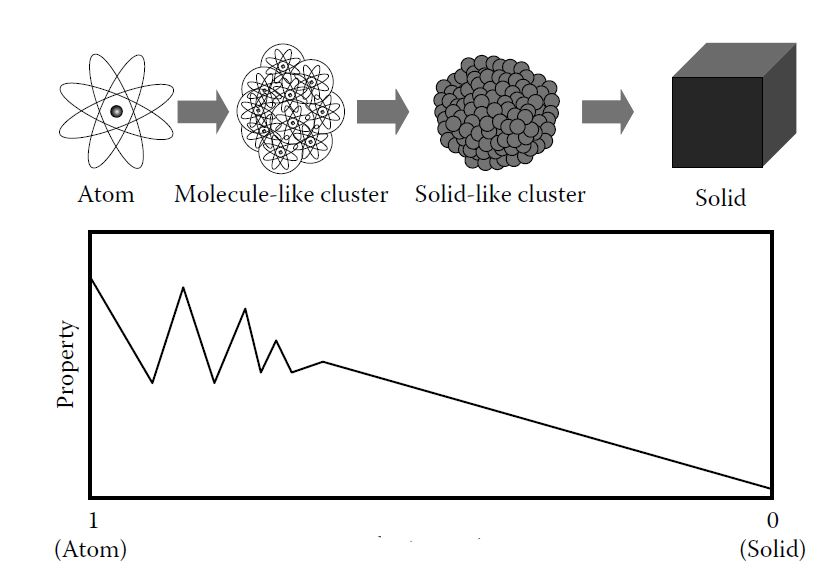
\includegraphics[width=0.7\textwidth]{images/clusters/atomo_cluste_solido}
  \caption{Esquema de transformação dimensional de átomos através de pequenos e grandes \textit{clusters} para o estado sólido. Quando os \textit{clusters} são pequenos cada átomo adicionado é importante, por isso as propriedades mudam
de forma abruptamente com o tamanho. Quando os \textit{clusters} se tornam grandes,
propriedades mudam suavemente\cite{cap06_Nanophysics}. Adaptado.  }
  \label{fig:transicao_cluster_solido}
\end{figure}




\begin{figure}
  \centering
  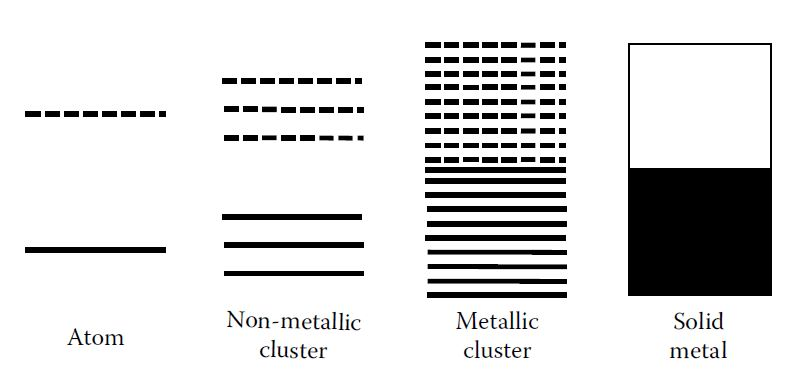
\includegraphics[width=0.65\textwidth]{images/clusters/carac_metal}
  \caption{ Esquema de transformação estrutural de energia a partir de átomos de metal através de pequenos e grandes \textit{clusters} para o metal sólido. Abaixo de um certo tamanho de \textit{clusters}, no qual as bandas vazia e povoada se fundem, um \textit{clusters} de átomos de metal pode ter uma estrutura de energia semelhante a um semicondutor.\cite{dissertacao_anderson}  }
  \label{fig:carac_metal}
\end{figure}

Os \textit{clusters} podem ser produzidos a partir de diversos elementos da tabela periódica, como por exemplo: metais alcalinos como sódio (Na), potássio (K); metais alcalinos-terrosos como cálcio (Ca), magnésio (Mg) e bário (Ba) metais nobres como ouro (Au), prata (Ag) e cobre (Cu). Quando estudados as nanopartículas de materiais que pertencem a mesma família as propriedades seguem o mesmo padrão.


\section{Espectro de massa das nanopartículas}

Em 1984, Knight et al \cite{electronic_Shell_sodium}, realizou um experimento com nanopartículas de sódio (Na), com N átomos por conglomerado (N = 4-100), e foram encontrado padrões, com picos bem definidos, no espectro de massa de \textit{clusters} de Na em fase gasosa, podendo ser visto na Figura \ref{fig:espec_na}(a). Cada pico do espectro representa o número de 
aglomerados de um determinado N detectado. Note a presença de picos maiores, quando comparado com os outros picos, para certas massas correspondentes à N = $8, 20, 40, 58$ e $92$, onde podemos notar padrões. 




\begin{figure}
  \centering
  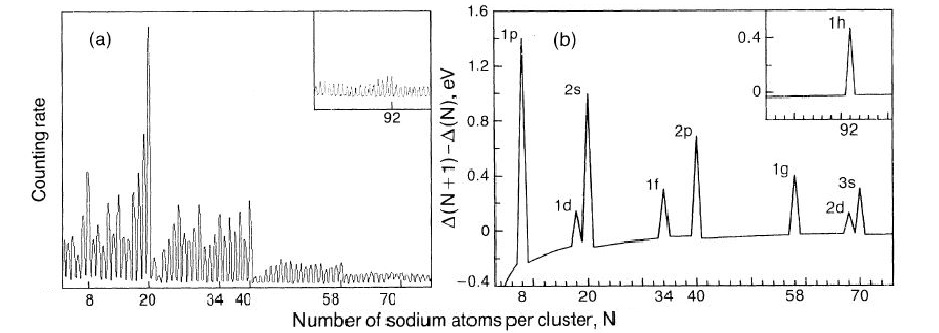
\includegraphics[width=1\textwidth]{images/clusters/NA_knight}
  \caption{(a) Espectro de massa de \textit{clusters} de sódio, N = 4-75.
  (b) A mudança calculada na diferença de energia eletrônica. Os picos protuberantes correspondem aos orbitais de casca fechada.\cite{electronic_Shell_sodium}  }
  \label{fig:espec_na}
\end{figure}


As características dos espectros de massa de outros metais alcalinos e também dos metais nobres, seguem um padrão semelhante ao do sódio.

Em 1985, Katakuse et al \cite{KATAKUSE1985229}, realizou um experimento com nanopartículas de cobre, prata e ouro, com $250$ átomos, e também foram encontrado padrões, com picos bem definidos em cada espectro de massa, como podemos ver nas Figuras \ref{fig:espec_ag},\ref{fig:espec_cu} e \ref{fig:espec_au}. No espectro de prata (Ag), podemos notar uma maior abundância nos picos como número de átomos iguais, $n= 3,9,21,35,41,59,93,139$ e $200$, já no espectro de cobre (Cu) vemos que a abundância dos picos são nos \textit{clusters} com $n= 3,9,21,35,41,59,93,139$ e no espectro de ouro (Au) vemos que a abundância dos picos são nos \textit{clusters} com $n= 3,9,21,35,59,93,139$.






\begin{figure}
  \centering
  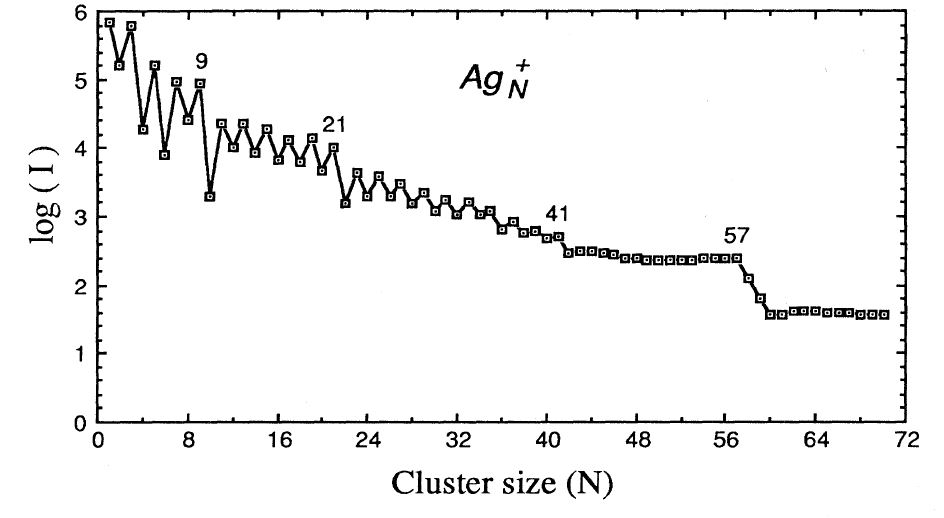
\includegraphics[width=0.7\textwidth]{images/clusters/espec_ag}
  \caption{(a) Espectro de massa de \textit{clusters} de prata \cite{Heer}.  }
  \label{fig:espec_ag}
\end{figure}

\begin{figure}
  \centering
  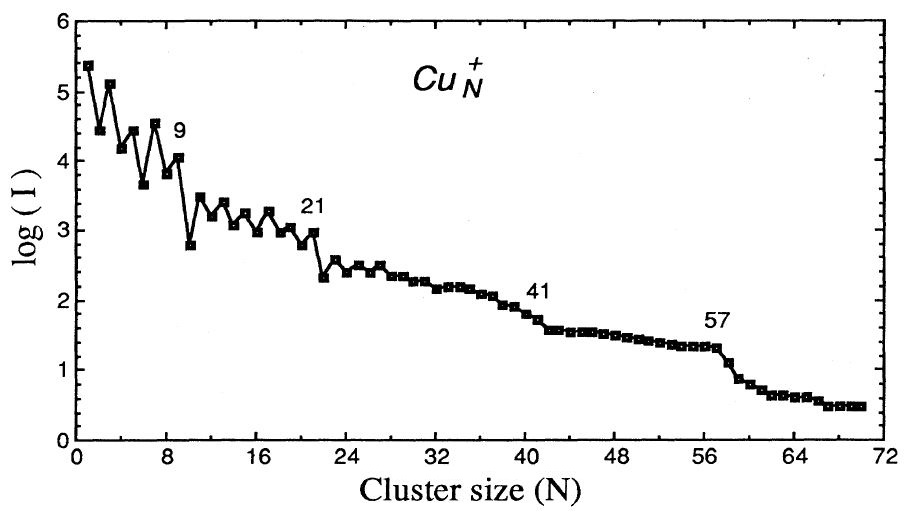
\includegraphics[width=0.7\textwidth]{images/clusters/espec_cu}
  \caption{(a) Espectro de massa de \textit{clusters} de cobre \cite{Heer}.  }
  \label{fig:espec_cu}
\end{figure}

\begin{figure}
  \centering
  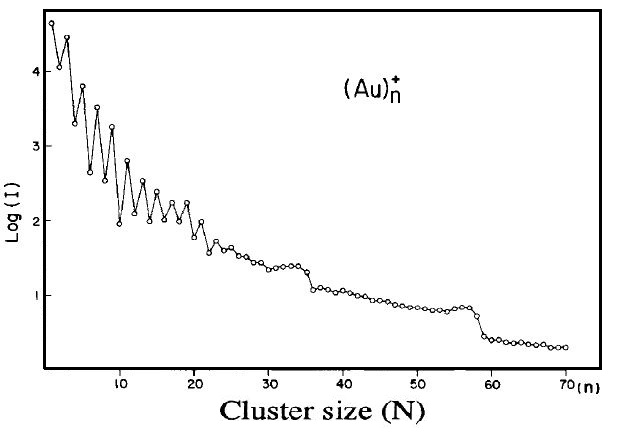
\includegraphics[width=0.65\textwidth]{images/clusters/espec_au}
  \caption{(a) Espectro de massa de \textit{clusters} de ouro \cite{KATAKUSE1985229}.  }
  \label{fig:espec_au}
\end{figure}




Os \textit{clusters} mais abundantes
nos espectros de massa, foram apelidados de \textit{clusters mágicos} ou \textit{clusters com números mágicos de átomos}, e são considerados relativamente mais estável. Podemos destacar a estrutura eletrônica dessas nanopartículas como a causa de maior estabilidade, como veremos a seguir.

Podemos explicar a ocorrência desses \textit{clusters mágicos} foi suposto o efeitos de preenchimento de camadas eletrônicas, em que a combinação entre o espectro de estados
quantizados e o princípio de exclusão de Pauli resulta em efeitos de camada \cite{Brack}. O modelo quântico de \textit{Jellium} \cite{Heer}, foi usado com sucesso para explicar a ocorrência desses \textit{clusters mágicos} \cite{capitulo_livro_shell}, como veremos na secção \ref{section_shell_model}.

Para as nanopartículas consideradas grandes, o padrão de números mágicos aparece diferente, e no geral ele é atribuído como uma consequência do preenchimento de camadas geométricas ou poliédricas de casca, assim o \textit{clusters} assume geometrias que minimizam a relação átomo-superfície uma vez que os átomos da superfície possuem um número menor de vizinhos do que os átomos internos, e o \textit{clusters} tende a preferir a estrutura de menor energia, maximizando a fração de átomo em massa. Essa estrutura geométrica da casca é bem conhecida nos \textit{clusters} de gás, e é característica de interações de curto alcance nas quais a tendência é para o empacotamento próximo do atomizado juntamente com a necessidade de minimizar a energia superficial \cite{capitulo_livro_shell}.


\section{Estrutura eletrônica \textit{shell model} para \textit{clusters} esféricos} \label{section_shell_model}

Pretendemos apresentar uma visão geral das características do sistema eletrônico \textit{shell model} ou modelo de concha.

O espectro de de massa da \ref{fig:espec_na} sugere que, os elétrons de valência nos \textit{clusters} de sódio são independentes e estão confinados em um potencial esfericamente simétrico. Assim como os átomos, as camadas eletrônicas de um \textit{cluster} com um número exato de elétrons para formar uma estrutura geometria poliédrica fechada, que o torna muito estável. Assim que um átomo for adicionado a nanoestrutura, seu elétron de valência ocupará um estado com energia maior e assim a estabilidade do \textit{cluster} será reduzida, ocasionando uma rejeição deste estado e reduzindo sua sua abundância no espectro e isso explica a grade abundância após cada número de fechamento da casca\cite{capitulo_livro_shell}.

Os números quânticos dos \textit{cluster} metálicos, são caracterizados de modo que cada casca possuí um número quântico radial \textit{n} e o momento angular \textit{l}. Para um dado número quântico \textit{l}, o estado mais baixo tem $n = 1$, e assim por diante.


Uma primeira aproximação com abordagem quântica, é o "Modelo de Gota" que fornece uma descrição boa do comportamento observado na Figura \ref{fig:espec_na}. O \textit{cluster} é representado como uma esfera de raio \textit{R}, que está relacionada com número \textit{N} de átomos e o raio de Wigner-Seitz, $r_{s}$\cite{capitulo_livro_shell}\cite{livro_cap16_Misra2012527}.


\begin{equation}
\label{eq:raio_R}
    R = r_{s}(N)^{\frac{1}{3}}
\end{equation}

O raio de Wigner-Seitz, $r_{s}$, é definido como o raio do volume ocupado por cada elétron de valência, isso é equivalente ao volume ocupado por cada átomo em um nanometal monovalente.
A estrutura interna do \textit{cluster} não é levada em consideração neste modelo. Este modelo é equivalente à teoria elétrons livre de sólidos. No entanto, a caixa sólida tem dimensões macroscópicas e níveis energéticos contínuos, enquanto o modelo para o \textit{cluster}, situado em nanoescala, os níveis de energia são discretos. Os primeiros níveis de energia para elétrons que não interagem em uma caixa esférica e o número de elétrons necessários para o preenchimento completo das camadas são $n= 2,8,18,20,34,40,58$ \cite{livro_cap16_Misra2012527}. Note que esses números condizem com os picos de maior abundância apontados no espectro da Figura \ref{fig:espec_na}.






Para o modelo de concha esféricas, os núcleos iônicos são substituídos por carga positiva uniforme de raio \textit{R}, os elétrons são tratados como partículas livres, movendo-se em um potencial parametrizado. O parâmetro básico do modelo é o raio de Wigner-Seitz, e a função onda para um potencial esfericamente simétrico pode ser escrita como:

\begin{equation}
    \psi_{ n,l,m}(r, \theta, \phi) = R_{nl}(r)Y_{lm}(\theta, \phi)
\end{equation}

Existem três potenciais úteis para o estudo da física de \textit{cluster}: potencial do oscilador harmônico, potencial esférico de poço quadrado e potencial Woods-Saxon. Estes potênciais são mostrados graficamente na Figura \ref{fig:pocos}.

\subsubsection{Potencial do Oscilador Harmônico:}

O potencial mais simples é o potencial do oscilador harmônico $V_{r}$:

\begin{equation}
    V(r)= \frac{1}{2}m\omega_0r^2
\end{equation}

o potencial do poço quadrado esférico (constante para $r<R$ e infinito para os demais). Como podemos ver na primeira coluna da Figura \ref{fig:pocos}, os níveis de energia para o potencial do oscilador harmônico são igualmente espaçados, altamente degenerados e são rotulados pelo número quântico \textit{v}.


A energia do potencial do oscilador harmônico é dada por:

\begin{equation}
    E_{v}= \left(\frac{3}{2}+v\right)h\omega_0
\end{equation}

Os números quânticos $(n,l)$ podem ser usados para qualquer potencial esfericamente simétrico. Assim, todos os orbitais com o mesmo valor de $(2n+l)$ são degenerados e as energias são escritas em termos do único número quântico $(2v+l-2)$. A energia potencial devido à carga de fundo é \cite{livro_cap16_Misra2012527}:
\begin{equation}
    \hbox{V}(r)
= \left\{ \begin{array}{lll}
\frac{3e^2N}{8\pi\epsilon_0R^3}\left(\frac{r^2}{3}-R^2\right) & \hbox{se} & r<R \\
e^2 Z & \hbox{} &  \\
\frac{e^2N}{4\pi\epsilon_0r} & \hbox{se} & r > R
\end{array}\right.
\end{equation}

\subsubsection{Potencial Esférico de Poço Quadrado:}

O potencial esférico de poços quadrados é descrito por:



\begin{equation}
 V(r) = \left\{\begin{array}{lll}
C & \hbox{se} & r < R \\
\infty & \hbox{se}  & \forall r
\end{array}\right.
\end{equation}




C é uma constante. A função de onda radial $R_{nl}(r)$ para o potencial do poço quadrado é escrita em termos da função de Bessel esférica $j_{l}(K_{nl}R)$, onde

\begin{equation}
    K_{nl}=\left[\frac{2m|E|}{\hbar^2}\right]^{\frac{1}{2}}
\end{equation}

Os níveis de energia são determinados pelas condições de contorno $j_{l}(K_{nl}R)=0$ e, para cada $l$, o primeiro zero de $j_l$ é dado o número quântico $n = 1$, o segundo $n = 2$, e assim por diante. A ordem dos níveis de energia (que são emprestados da física nuclear e são diferentes da física atômica) são $1s$, $1p$, $1d$, $2s$, $1f$, $2p$, $1g$, $2d$,... Se duas soluções tiverem o mesmo número de nós radiais, aquela com maior $l$ terá maior energia. Nesta notação, o número quântico principal em física atômica é igual a $n + l$. O interior do \textit{cluster} será eletricamente neutro se incluirmos a contribuição da correlação de troca para o potencial eletrostático dos elétrons, e o potencial efetivo será quase constante. O potencial do poço quadrado representa essencialmente esse fenômeno\cite{livro_cap16_Misra2012527}.


\subsubsection{Potencial de Woods–Saxon:}

Em seu artigo Knight et al\cite{electronic_Shell_sodium} utiliza o potencial de Woods-Saxon, para realizar a análise dos espectros de massa de sódio mostrados na Figura \ref{fig:espec_na}\cite{livro_cap16_Misra2012527}, uma vez que ele é o potencial que melhor produz uma representação fenomenológica um potencial plano no centro de \textit{cluster} arredondado nas bordas. Este potencial é descrito por:

\begin{equation}
    U(r)=\frac{-U_0}{exp[(r-R)/\epsilon]+1}
\end{equation}


$U_0$ é a soma da energia de Fermi e a função de trabalho do metal a granel. $R$ é determinado pela \ref{eq:raio_R}. O parâmetro $\epsilon$ é usado para corresponder à variação do potencial na superfície. Para este potencial, não existem soluções analíticas.


Uma comparação entre os três potenciais apresentados, pode ser vista na Figura \ref{fig:pocos}. Nela podemos ver que a degenerescência dos estados do potencial Woods-Saxon é semelhante à do potencial do poço quadrado, mas a ordenação dos níveis de energia são diferentes.

 Note também que os níveis com o mesmo momento angular são interligados. Pode-se ver que a sequência de níveis dependem do potencial radial. Isso influi nos números “mágicos”, ou seja, nos números de elétrons para os quais os \textit{clusters} são especialmente estáveis. Nos níveis, os números de elétrons acumulados são dados: 2 elétrons preenchem o nível $1s$, 8 elétrons preenchem as camadas $1s$ e $1p$ e assim por diante.
 
 Os \textit{clusters} mais estáveis são aqueles com um nível completamente preenchido (chamado de casca fechada) e um grande espaço entre o nível ocupado mais alto e o nível mais baixo não ocupado. Portanto, os números de elétrons $34$ e $58$ são números “mágicos” do potencial quadrado, mas não do potencial Woods–Saxon. Os números $20$ e $40$ são fortemente “mágicos” para o oscilador harmônico e o potencial Woods–Saxon, mas menos para o potencial da caixa. Então, quais tamanhos de \textit{clusters} são especialmente estáveis depende fortemente do potencial radial, que pode ser diferente para diferentes metais.
 
Os números observados para sódio
\textit{clusters} na Figura \ref{fig:espec_na} $(8, 20, 40, 58)$ indicam que o potencial efetivo de partícula única está entre uma caixa e um potencial Woods–Saxon. Mas o mais importante é o acordo desses números com as previsões do modelo simples, o modelo de elétrons livres é capaz de descrever sistema eletrônico de \textit{clusters} de sódio \cite{livro_Clusters_Fullerenes}.

\begin{figure}
  \centering
  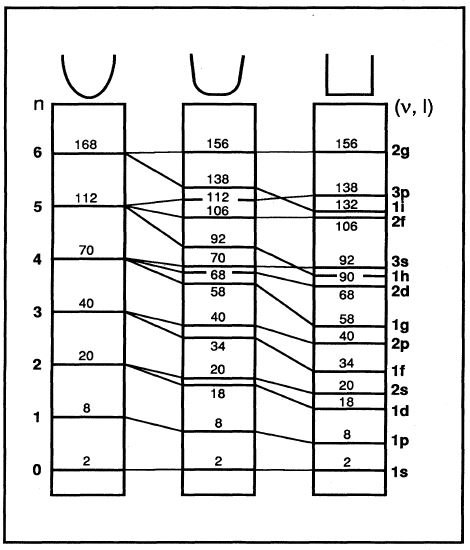
\includegraphics[width=0.5\textwidth]{images/clusters/pocos}
  \caption{Comparação dos potenciais (a) harmônico, (b) Woods-Saxon e (c) poço quadrado. \cite{Heer}}
  \label{fig:pocos}
\end{figure}

Em contra partida, os "números mágicos" para os espectros de prata, cobre e ouro, mostrados nas Figuras \ref{fig:espec_ag},\ref{fig:espec_cu} e \ref{fig:espec_au}, ocorrem
$9, 21, 35,...$ , diferente dos \textit{clusters} de sódio. Eles possuem as camadas 3d, 4d e 5d, com a camada d preenchido com 10 elétrons e um único elétron de valência. No experimento de Katakuse et. al. 1985,  os \textit{clusters} foram produzidos carregados positivamente, e assim o número de elétrons em um aglomerado era $N - 1$, desta forma os números mágicos correspondentes às cargas eletrônicas de conchas estão coerentes com os resultados experimentais \cite{Heer}.

Comparando os espectros de sódio com os espectros dos metais nobres apresentados, vemos que neles a estrutura fina é dominada por um alternância par-ímpar nas intensidades, enquanto o espectro de sódio reflete a estrutura da subcamada prevista neste modelo. 





\chapter{Materiais e Métodos}
\label{c3}


A produção de \textit{clusters} é suportada basicamente por duas técnicas: \textit{top-down} e \textit{bottom-up}. Na primeira, a partir de um material com dimensões macroscópicas, as nanoestruturas são formadas a partir da remoção deste material utilizando técnicas como feixe de elétrons ou litografia de feixe de íons focalizado. Na segunda técnica, as nanopartículas são produzidas por síntese química, e então a organização entre elas se da por propriedades físicas ou químicas.

A produção de nanopartículas por síntese química é mais simples porém o controle de pureza torna-se mais complicado. O método de produção por síntese física (\textit{top-down}), requer um aparato experimental sofisticado, que será apresentado neste capítulo, porém o controle de pureza dos \textit{clusters} é altamente preciso.





\section{A Fonte de \textit{Clusters} e Agregados}

A Fonte de \textit{Clusters} e Agregados (FoCA), esquematizada na Figura \ref{fig:esquema_foca}, produz nanopartículas metálicas que variam entre $1$ podendo chegar $40.000$ átomos (ou $5nm$, no caso da prata), essa produção se da por método físico, mais especificamente \textit{sputtering}.

O funcionamento da máquina ocorre basicamente em quatro etapas: primeiramente uma nuvem de átomos é produzida por um \textit{sputtering}; em seguida, são resfriadas por nitrogênio líquido ocorrendo a agregação dos átomos em nanopartículas na presença do gás argônio; na sequência, o feixe de agregados, carregados eletricamente, é guiado por um conjunto de lentes eletrostáticas até chegar no espectrômetro de massa por tempo de voo, onde $\approx10\%$ do feixe é desviado para a análise do espectro de distribuição de massa, sendo possível identificar a massa e por consequência o tamanho das partículas produzidas, por fim as nanopartículas são depositadas no porta amostras. Na Figura \ref{fig:foto_foca} podemos ver uma foto real da máquina. 

\begin{figure}
  \centering
  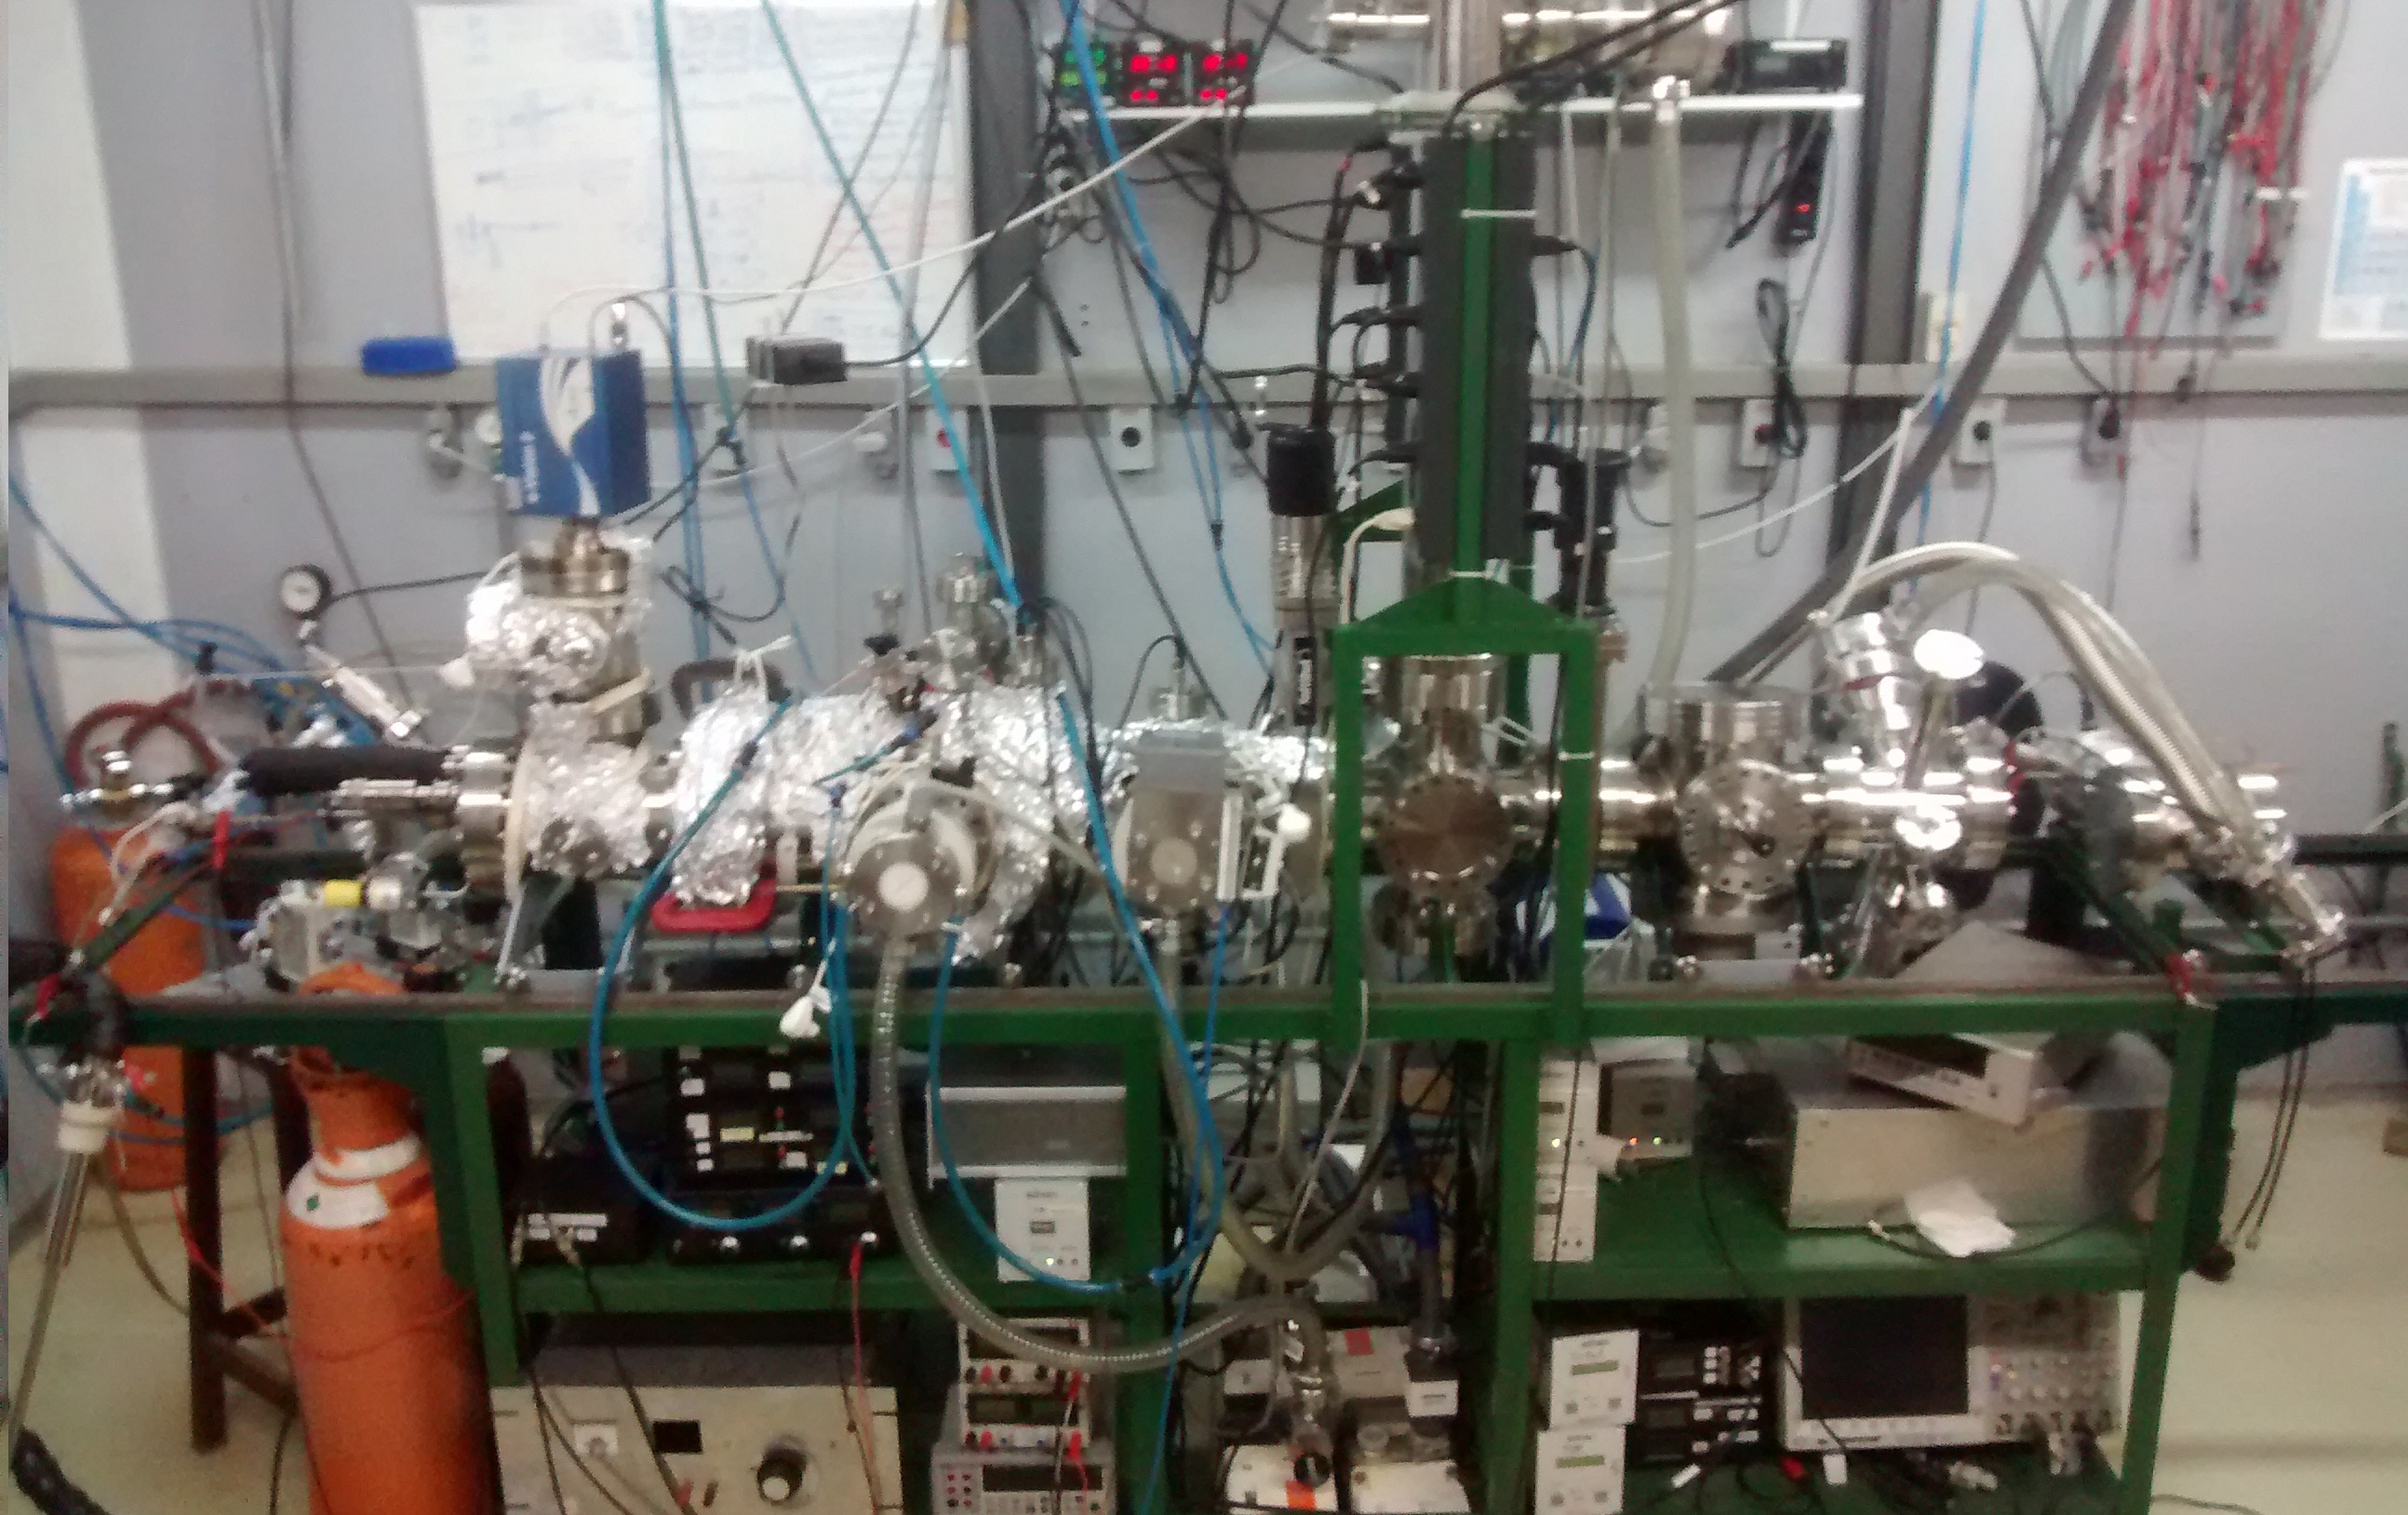
\includegraphics[width=0.7\textwidth]{images/foca/foto_foca}
  \caption{ Imagem real da  Fonte de \textit{Clusters} e Agregados.  }
  \label{fig:foto_foca}
\end{figure}

\begin{figure}
  \centering
  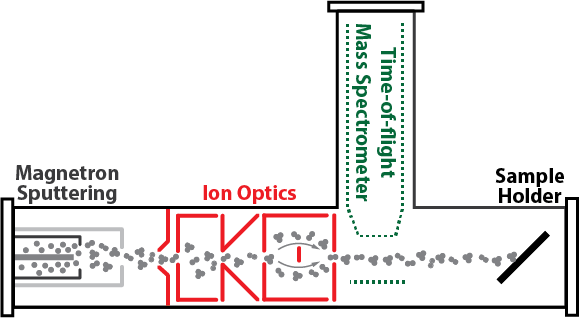
\includegraphics[width=0.8\textwidth]{images/foca/esquematico_foca}
  \caption{ Diagrama da fonte de Fonte de \textit{Clusters} e Agregados. ``\textit{Magnetron Sputtering}'' é a fonte de átomos que se encontra dentro da câmara de agregação. Depois de produzido e agregado, o feixe passa por um conjunto de lentes eletrostásticas  ``\textit{Ion Optics}''. Uma parte do feixe é desviado para o ``\textit{Time-of-flight Mass Spectrometers}'' (ToF), onde é realizada a aquisição do espectro de voo, outra parte é depositada na amostra "\textit{Sample Holder}"\cite{livro_vitor}.  }
  \label{fig:esquema_foca}
\end{figure}

As lentes eletrostáticas possuem as seguintes funções: focalizar o feixe de íons, retirar as partículas neutras, de acordo com o potencial aplicado nas lentes elas também podem funcionar com um filtro em função das energias das partículas. As lentes consistem de uma série de eletrodos de simetria cilíndrica nas quais são aplicadas potenciais. Uma foto das lentes pode ser vista na Figura \ref{fig:foto_lentes}.

\begin{figure}
  \centering
  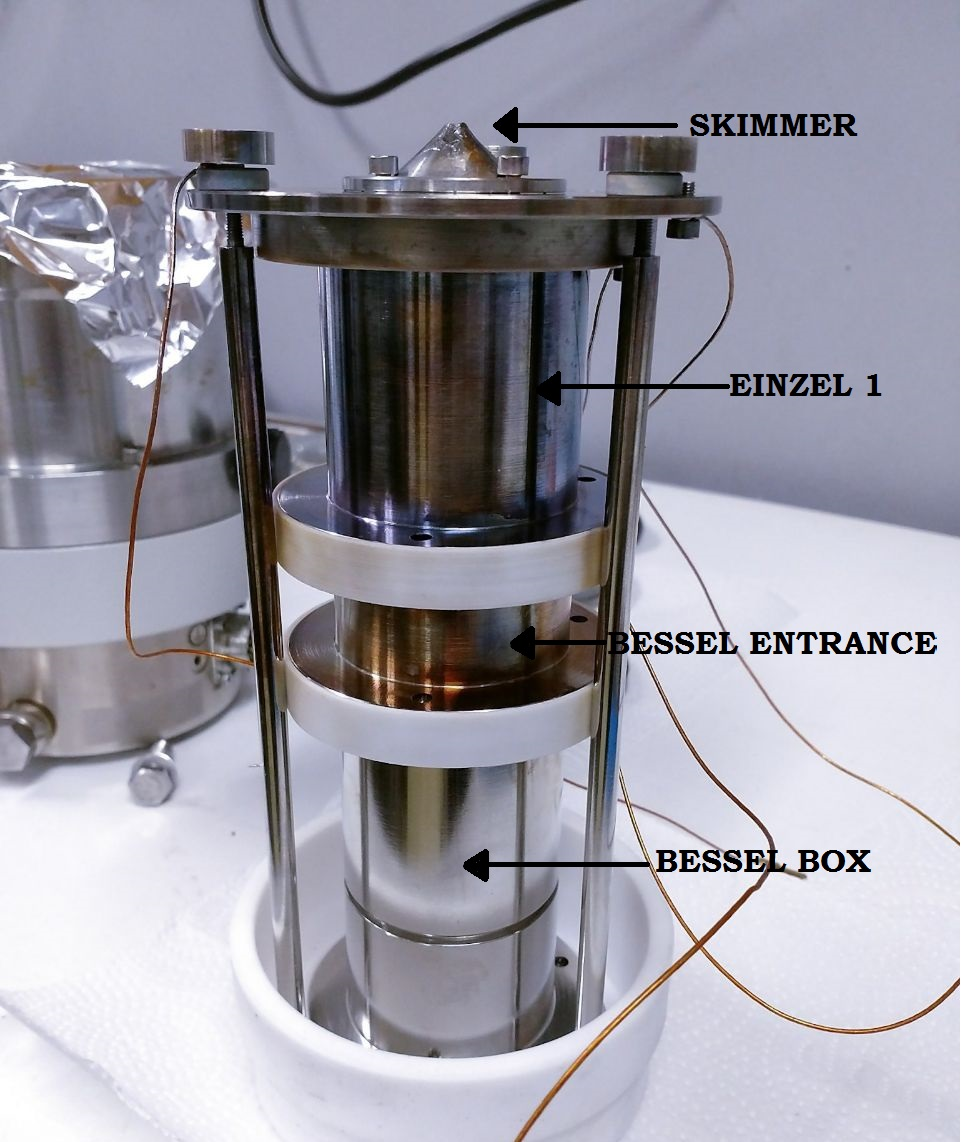
\includegraphics[width=0.6\textwidth]{images/foca/lentes}
  \caption{ Foto da lentes eletrostáticas.  }
  \label{fig:foto_lentes}
\end{figure}



Existem muitas formas de síntese de nanopartículas, seja por método químico ou físico. Como exemplo da primeira, para o caso da prata, podemos citar a redução com borohidreto de sódio e como exemplo da segunda, agora em um caso mais geral de metais, podemos citar a evaporação térmica e a técnica de \textit{sputtering} ou pulverização catódica.

Para gerar nossa nuvem de átomos, a FoCA utiliza um \textit{magnetron cilíndrico} \cite{ref_artigo_foca}, que caracteriza a produção desses \textit{clusters} por \textit{sputtering}, aqui o alvo, material que dará origem às nanopartículas, possuí o formato de um fio e fica localizado no eixo do \textit{magnetron}.

A versatilidade dessa técnica encontra-se no fato que o alvo é multivalente, podendo ser composto de vários metais, incluindo ligas, como por exemplo a mistura ouro e prata, bastando entrelaçar os fios do metal de desejo para isso. Na Figura \ref{fig:magnetron} podemos ver o plasma gerado no \textit{magnetron cilíndrico}. Pela presença de um campo elétrico os íons são acelerados em direção ao alvo do metal de interesse e o corrói. Na Figura \ref{fig:alvo} é possível observar um alvo de prata, composto por um único fio, novo e ao lado um já erodido.

\begin{figure}
  \centering
  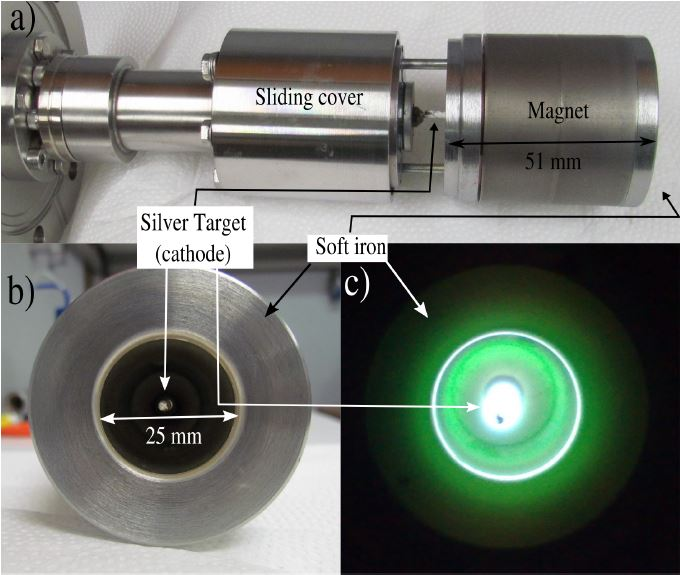
\includegraphics[width=0.75\textwidth]{images/foca/magnetron_cil}
  \caption{ (a) Magnetron cilíndrico oco caseiro com a tampa deslizante retraída para mostrar o alvo de prata. (b) vista frontal. (c) Vista frontal com plasma aberto. Observe a cor esverdeada ao redor do alvo, tipicamente vista na formação de plasma prateado.\cite{livro_vitor} }
  \label{fig:magnetron}  
\end{figure}


\begin{figure}
  \centering
  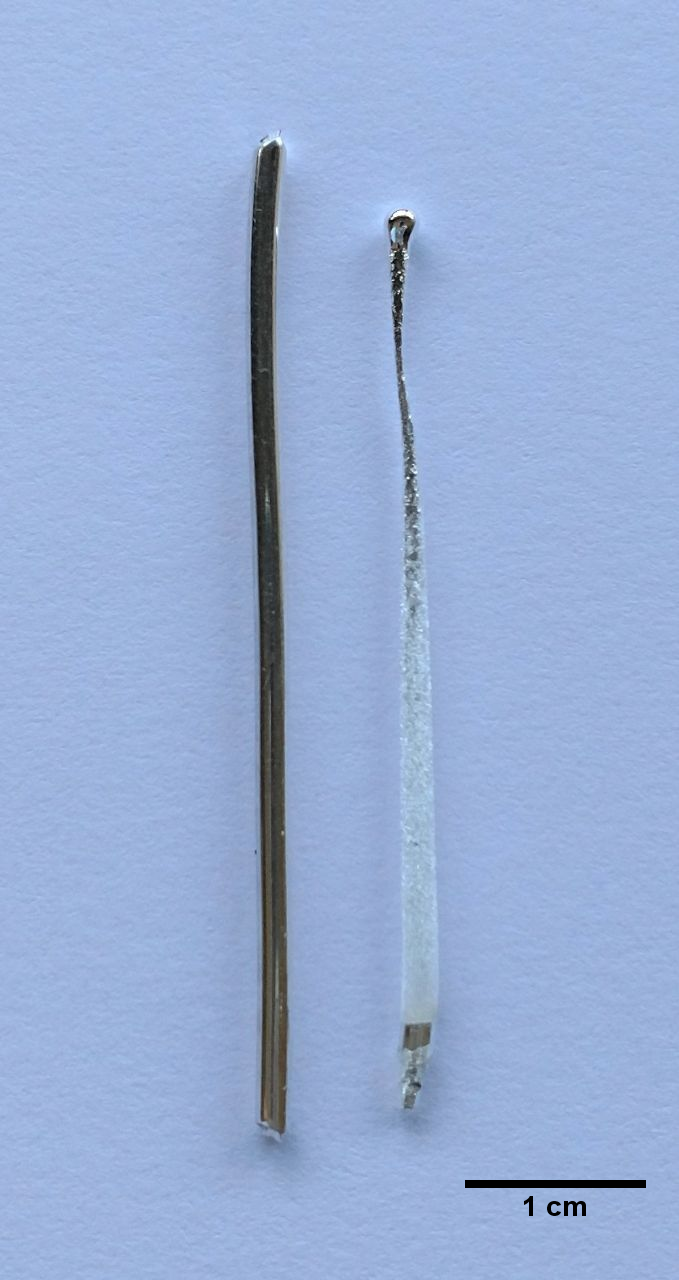
\includegraphics[width=0.3\textwidth]{images/foca/alvo}
  \caption{ Foto de um alvo de prata de fio único. À esquerda temos um alvo novo e à direita temos um alvo já corroído.  }
  \label{fig:alvo}
\end{figure}






\section{Espectrômetro de massa por tempo de voo}

Esta seção será dedicada a descrever o princípio de funcionamento da técnica de \textit{Time-of-flight Mass Spectrometers} (TOFMSs).

Na Figura \ref{fig:tof}, pode-se observar o esquema do espectrômetro, onde o pulso elétrico fornece velocidade perpendicular ao feixe de partículas carregadas, que viajam dentro de um tubo de voo - livre de variação de potencial elétrico - até encontrarem um detetor de corrente. Por sua vez, o detetor faz a contagem de íons em função dos tempos de chegada.

O TOFMSs funciona  baseado no fato de que, ao receber a mesma quantidade de energia fornecida por um campo elétrico pulsado, partículas com massas diferentes adquirem velocidades distintas \cite{dissertacao_kevin}. Assim, as partículas mais leves atingirão o detector antes das partículas mais pesadas.

\begin{figure}
  \centering
  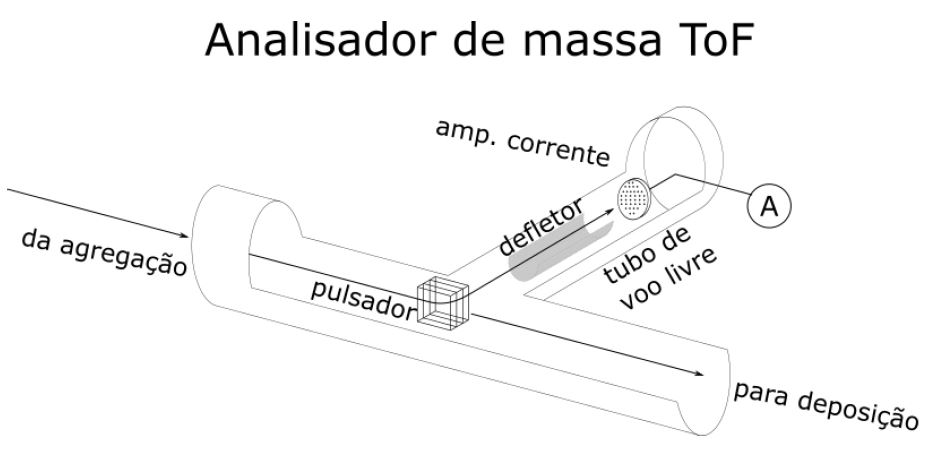
\includegraphics[width=1\textwidth]{images/foca/tof}
  \caption{ O pulsador é um conjunto de placas com campo pulsado, que confere uma velocidade perpendicular ao feixe de partículas eletricamente carregadas. Os defletores impedem que as partículas colidam com as paredes do tubo de voo livre. ``\textit{A}'' representa o detector de corrente, cuja função é realizar a contagem dos íons em função do tempo de chegada.  \cite{dissertacao_kevin}.  }
  \label{fig:tof}
\end{figure}

Para calcular o tempo de voo, vamos considerar um \textit{cluster} de massa $m$ e carga $q$. O campo elétrico vai fornecer energia cinética ($K = qV$) para a partícula, em que $V$ é a voltagem fornecida pelo pulsador. Assim, é possível expressar a velocidade da partícula como:

\begin{equation}
v = \sqrt[]{\frac{2qV}{m}}
\end{equation}

O detector de corrente está situado a uma distância $L$ da região onde a partícula adquire velocidade. Note que essa partícula levará um tempo $t_{voo}$ para atingir o detector, e esse tempo pode ser calculado por:

\begin{equation}
\label{eq:tempo_voo}
t_{voo} = L \cdot \sqrt[]{\frac{1}{2V} \frac{m}{q}} 
\end{equation}


A corrente que chega ao detector é convertida em tensão por um amplificador IV, e o sinal é exibido em um osciloscópio, e então para aquisição dos dados utiliza-se um programa desenvolvido pelo grupo.

A variável $L$ possui o valor de um metro, o potencial aplicado é de $V = 7 $  kV, e o tempo de voo das partículas é fornecido pelo osciloscópio, possibilitando calcular a massa das partículas.

Note que utilizando a Equação \ref{eq:tempo_voo} é possível também calcular o $t_{voo}$ de uma partícula se soubermos a massa. Vamos fazer uma análise para o caso de um átomo de prata. Segundo a tabela periódica um átomo de prata possui uma massa de $107,87$ unidades de massa atômica, convertendo sua massa para quilos temos $1,79\times 10^{-25}$ kg. A carga de partícula é a carga elementar de um elétron $1,60\times 10^{-19}$ C, e então seu tempo de voo vai ser aproximadamente$17,6$ $\mu$s.

Podemos também escrever a massa de uma nanopartícula em função da massa de uma outra partícula da qual conhecemos a massa e o tempo de voo.

\begin{equation}
\label{eq:relacao_massa_tempo}
M = \left(\frac{t}{t'}\right)^2 \cdot M'
\end{equation}


É possível estabelecer uma relação que futuramente vai permitir diferenciar outros picos de prata, e então calibrar o espectro de partículas produzido, confirmando o que foi depositado na amostra.


A grande vantagem desse tipo de técnica, espectrometria de massa por tempo de voo, é que a obtenção da distribuição de tamanhos produzida é exibida em tempo real, assim qualquer deformidade indesejável no espectro é passível de correção ainda durante o processo de deposição, por meio de ajuste  dos parâmetros da máquina. 

\section{Experimentos com luz ultravioleta}

Para realizar experimentos com incidência de luz ultra violeta, foi preciso montar um sistema de iluminação, que consiste em inserir um LED do UV, modelo UVTOP240 TO39 produzido pela Roithner Lasertechnik GmbH, na fonte de agregados. Para isto foi instalado um passante de tensão para que o LED fique em dentro da máquina. Além disso, um sistema de alimentação, com controle de corrente, foi montado utilizando uma fonte de tensão.

O LED é baseados em AlGaN (Alumínio, Gálio e Nitrogênio), com um pico típico de comprimento de onda de $245 nm$ e potência de saída óptica de $30-70 \mu W$. Seu encapsulamento é metálico e hermeticamente fechado, com configuração de lente de vidro plano. Uma foto desse diodo pode ser vista na Figura \ref{fig:foto_led}.

\begin{figure}
  \centering
  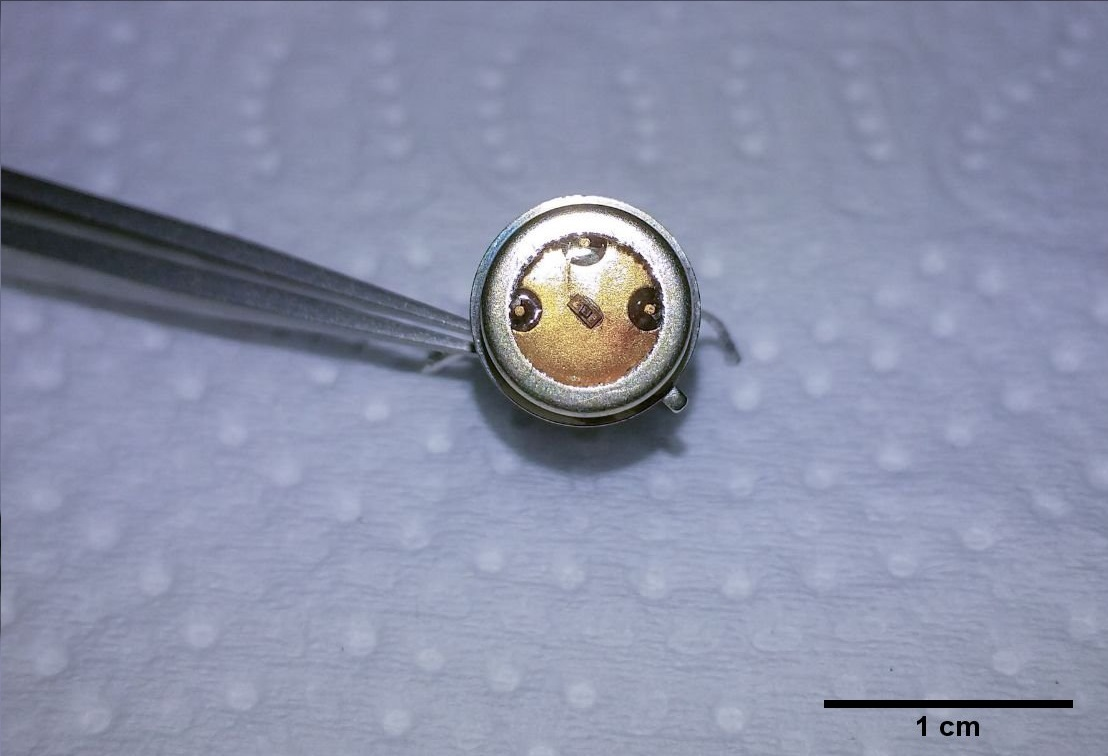
\includegraphics[width=0.7\textwidth]{images/foca/led_scale}
  \caption{ Foto do LED do UV, modelo UVTOP240 TO39, utilizado para ionização das nanopartículas.  }
  \label{fig:foto_led}
\end{figure}


Foi escolhido posicionar o LED entre saída da câmara de agregação e a primeira lente eletrostática, como podemos ver na Figura \ref{fig:led_montagem}. Os testes do aparato consistem na aquisição da corrente de agregados produzidos e do seu espectro de massa sem o uso do LED e posteriormente com o LED. Com isso foi avaliado o possível aumento de ionização, como a incidência de luz afeta o espectro de massa do sistema de agregação e possíveis ajustes nos valores da tensões das lentes eletrostáticas.
Assim, foram realizados experimentos com incidência de luz ultra violeta (UV), induzindo a sua ionização, e comparar os espectros de abundância obtidos com e sem o uso da luz UV. 



\begin{figure}
  \centering
  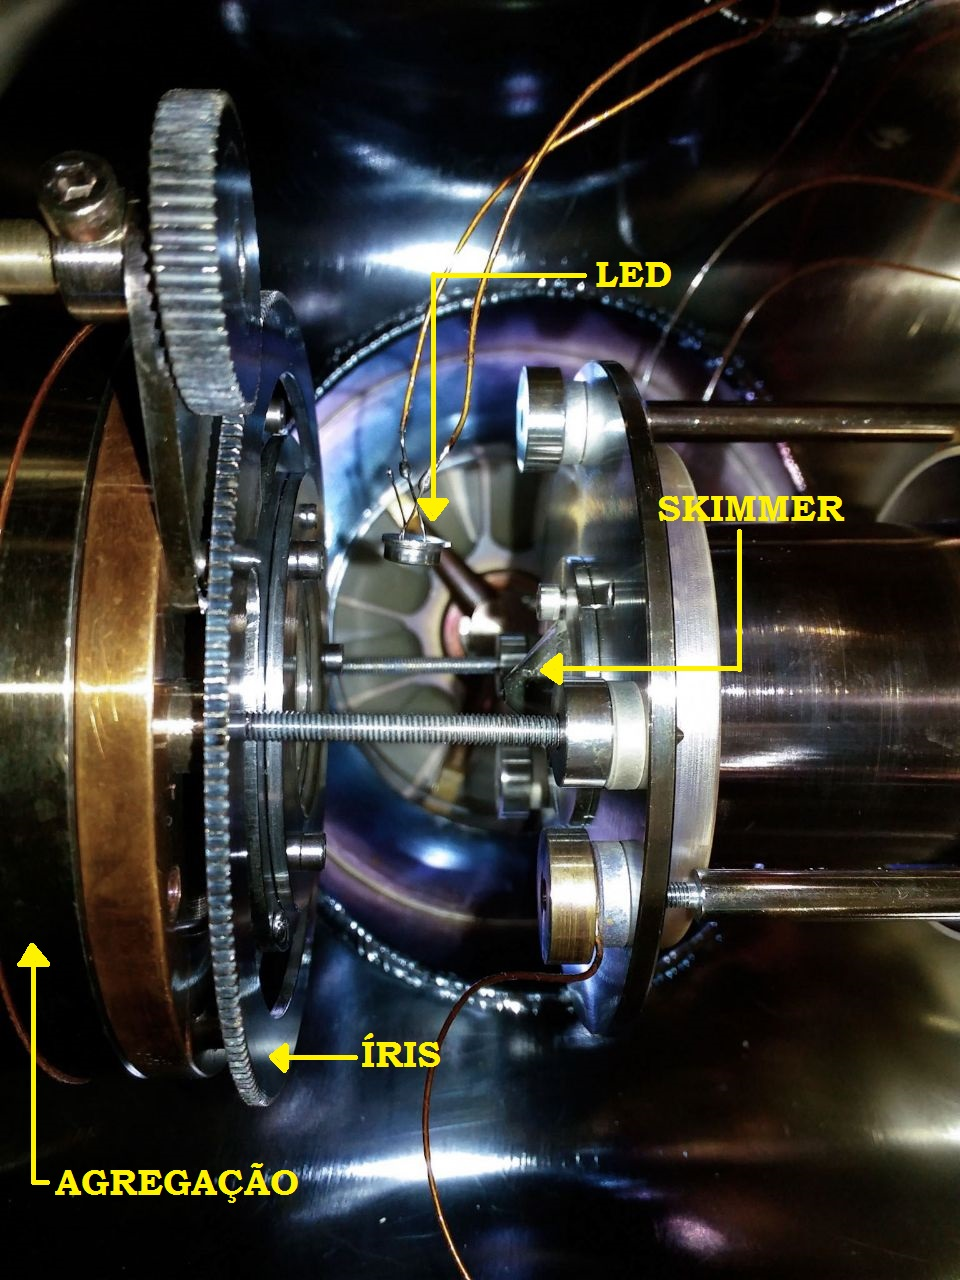
\includegraphics[width=0.7\textwidth]{images/foca/led_montagem}
  \caption{Foto do posicionamento do LED, localizado entre a câmara de deposição e a primeira lente eletrostática, Skimmer. Também está indicado a íris, peça que controla a pressão na câmara de agregação.}
  \label{fig:led_montagem}
\end{figure}








%\chapter{Conclusões} \label{conclusões}


%% \bibliography{./nsav}
%% \bibliographystyle{unsrt}
\addcontentsline{toc}{chapter}{Bibliografia}
\bibliographystyle{acm}
\bibliography{references.bib}


%\chapter*{Apêndices}
%\markboth{Apêndices}{Apêndices}
%\addcontentsline{toc}{chapter}{Apêndices}


%\appendix
%\title{Apêndices}

%\chapter{Condições de contorno}

%Para simular o hélio nas fases líquida e sólida nas densidades estudadas, utilizamos uma caixa de simulação com 64 ou 108

%\section{Janzen e colaboradores - $V_{pr}$}

%Os valores dos parâmetros para este potencial são os mesmos que para o 

\end{document}


